
%(BEGIN_QUESTION)
% Copyright 2014, Tony R. Kuphaldt, released under the Creative Commons Attribution License (v 1.0)
% This means you may do almost anything with this work of mine, so long as you give me proper credit

Examine this single-line diagram of a power distribution system, showing transformers, generators, circuit breakers, power lines, and some of the protective relays that would make a complete system.  In particular, pay close attention to {\it protection zones} for each relay, noting which pieces of equipment in this power system are protected by which relay:

$$\includegraphics[width=15.5cm]{i03099x01.eps}$$

\filbreak

Identify which relay(s) would command which circuit breakers to trip given the following faults:

\begin{itemize}
\item{} Phase-to-ground fault on the left-hand transmission line
\vskip 10pt
\item{} Phase-to-phase fault on the right-hand transmission line
\vskip 10pt
\item{} Loss of mechanical driving power for the middle generator
\vskip 10pt
\item{} Internal winding fault in right-hand generator transformer
\vskip 10pt
\item{} Phase-to-phase fault on the generator bus
\end{itemize}

\underbar{file i03099}
%(END_QUESTION)





%(BEGIN_ANSWER)

 
%(END_ANSWER)





%(BEGIN_NOTES)

\begin{itemize}
\item{} Phase-to-ground fault on the left-hand transmission line: {\it 87 relay tripping breakers G and J}
\vskip 5pt
\item{} Phase-to-phase fault on the right-hand transmission line: {\it 87 relay tripping breakers H and K}
\vskip 5pt
\item{} Loss of mechanical driving power for the middle generator: {\it 67 relay tripping breaker B and/or E}
\vskip 5pt
\item{} Internal winding fault in right-hand generator transformer: {\it 87 relay tripping breakers C and F}
\vskip 5pt
\item{} Phase-to-phase fault on the generator bus: {\it 87 relay tripping breakers D, E, F, G, and H}
\end{itemize}





\filbreak \vskip 20pt \vbox{\hrule \hbox{\strut \vrule{} {\bf Virtual Troubleshooting} \vrule} \hrule}

\noindent
{\bf Predicting the effect of a given fault:} present each of the following faults to the students, one at a time, having them comment on all the effects each fault would produce.

\begin{itemize}
\item{} Mild, persistent overcurrent condition at one of the loads on the bottom distribution feeder
\item{} Internal winding fault (to ground) on left-hand substation transformer
\item{} Catastrophic fault at one of the loads on the bottom distribution feeder
\item{} Loss of excitation in the field winding of the right-hand generator
\item{} Phase-to-ground fault on the generator bus
\item{} Internal phase-to-ground fault within circuit breaker \#3
\end{itemize}


\vskip 10pt


\noindent
{\bf Identifying possible/impossible faults:} present symptoms to the students and then have them determine whether or not a series of suggested faults could account for all the symptoms, explaining {\it why} or {\it why not} for each proposed fault:

\begin{itemize}
\item{} Symptom: {\it Circuit breakers 11, 12, and K tripped}
\item{} Ground fault in upper distribution feeder -- {\bf No}
\item{} Internal fault in circuit breaker \#8 -- {\bf No}
\item{} Internal ground fault in East bus transformer -- {\bf Yes}
\item{} Internal turn-to-turn fault in East bus transformer -- {\bf Yes}
\item{} Overload condition on one of the distribution feeders -- {\bf No}
\item{} Transmission line fault -- {\bf No}
\end{itemize}










\vfil \eject

\noindent
{\bf Summary Quiz:}

Suppose the middle generator suffered a loss of field excitation power, but its 40 relay failed to pick up.  Which other protective relay in this diagram could serve as a back-up to trip the generator's breaker and isolate it from the rest of the power system?

$$\includegraphics[width=15.5cm]{i03099x01.eps}$$

%INDEX% Electric power systems: single-line diagram
%INDEX% Electric power systems: zones of protection

%(END_NOTES)


